% -  -  -  -  -  -  -  -  -  -  -  -  -  -  -  -  -  -  -  -  -  -  -  -  -  -  -  -  -  -  -  -  -  -  -  -  -  -  -  -  -  -  -  -  -  -  -  -  -  -  -  -  - %
%-----Chapter 3: Kalman Filtering-------%
\chapter{Kalman Filtering}

\section{Linear Kalman Filter}
There exists a recursive Kalman filter algorithm for discrete time systems.\cite{IntroKF} This ongoing Kalman filter cycle can be divided into two groups of equations: \newline
\begin{enumerate}
	\item Time update equations
	\begin{equation}\label{TupEq}
		\begin{aligned}
    			\hat{x}_{k}^{-} &=& A\hat{x}_{k-1}+Bu_{k-1} \\
    			P_{k}^{-} &=& AP_{k-1}A^{T}+Q
  		\end{aligned}
	\end{equation}
	\item Measurement update equations
	\begin{equation}\label{MupEq}
		\begin{aligned}
    			K_{k} &=& P_{k}^{-}H^{T}(HP_{k}^{-}H^{T}+R)^{-1} \\
    			\hat{x}_{k} &=& A\hat{x}_{k-1}^{-}+K_{k}(z_{k}-H\hat{x}_{k}^{-}) \\
			P_{k} &=& (I-K_{k}H)P_{k}^{-}
  		\end{aligned}
	\end{equation}
\end{enumerate}

To test this algorithm and to learn something about applying the Kalman filter on linear system we created an example. A detailed description of the following example can be found in appendix \ref{ExampleKF}. \newline 
We consider a linear, timeinvariant model, given by the following circuit diagram in Figure \ref{KFcircuit}.
\begin{figure}[htbp]
	\centering
	\begin{pspicture}(-3,-1)(9,5)
		%nodes
			\pnode(-2,4){A}		\pnode(-2,0){B}		\pnode(8,4){C0}		\pnode(8,0){D}
			\pnode(3,4){A2}		\pnode(3,2){M}		\pnode(3,0){B2}	\pnode(6,4){C2}
			\pnode(6,0){D2}
		%elements
			\coil[intensitylabel=$i_L$,labeloffset=-0.2](A)(A2){$L$}
			\capacitor[tensionlabel=$U_1$,tensionlabeloffset=-1.2,tensionoffset=-0.8,%
					intensitylabel=$i_1$,dipoleconvention=generator](A2)(M){$C_1$}
			\resistor[tensionlabel=$U_R$,tensionoffset=0.8,labeloffset=-0.5](B2)(M){$R$}
			\capacitor[tensionlabel=$U_2$,tensionlabeloffset=-1.2,tensionoffset=-0.8,%
					intensitylabel=$i_2$,dipoleconvention=generator](C2)(D2){$C_2$}
		%wires
			\wire(B)(D)		\wire(A2)(C0)
			\pscircle[fillstyle=solid](A){0.075}
			\pscircle[fillstyle=solid](B){0.075}
			\pscircle[fillstyle=solid](C0){0.075}
			\pscircle[fillstyle=solid](D){0.075}
		%tension
			\tension(A)(B){$U_{in}$}
			\tension(C0)(D){$U_{out}$}
	\end{pspicture}
    	%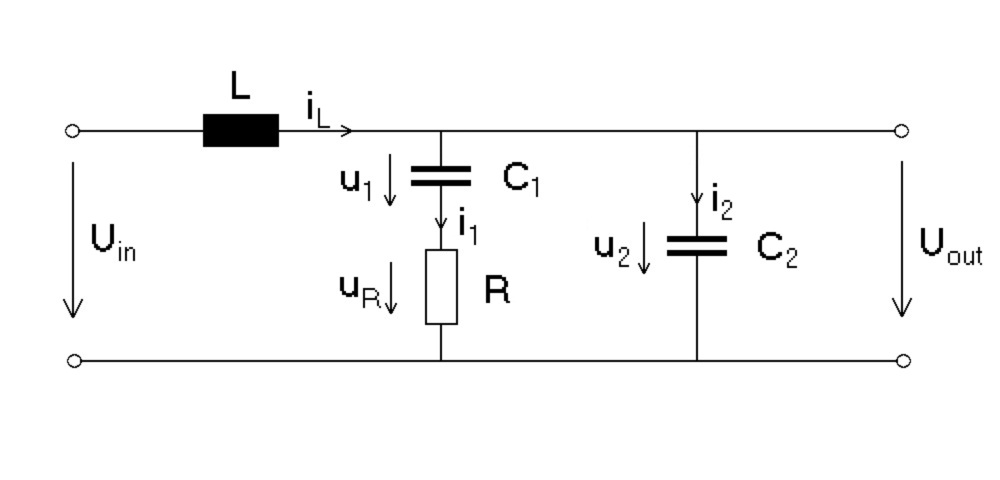
\includegraphics[width=12cm]{./3_KalmanFilter/circuit_diagram.jpg}
  	\caption{Example: Linear electrical circuit.}
  	\label{KFcircuit}
\end{figure}
First we added process noise and measurement noise to the system output. The aim is to get an estimation of the noisy output. Therefore we applied the Kalman filter algorithm based on the equations \ref{TupEq}. In the figure \ref{KFchart}, above we can see the input signal and the ideal measurement of the output signal. That ideal measurement includes process noise, which can obviously not be filtered by the Kalman filtering algorithm. Below one can see the noisy measurement on the left side and the filtered output on the right side.
\begin{figure}[htbp]
	\centering
    	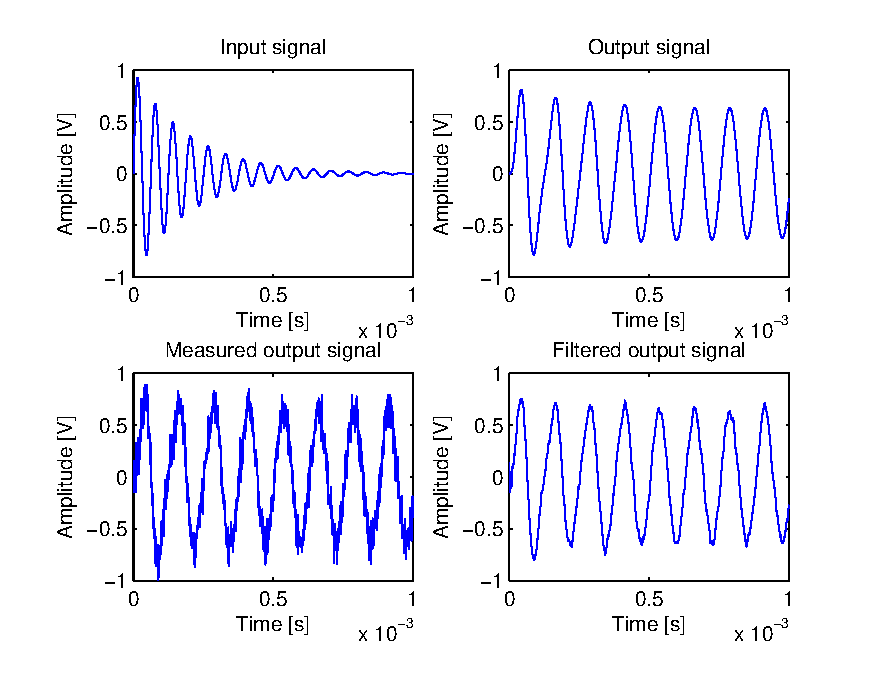
\includegraphics[width=12cm]{./3_KalmanFilter/KFchart}
  	\caption{Example: Input signal, output signal, noisy output, and filtered ouptut.}
  	\label{KFchart}
\end{figure}

\section{Extended Kalman Filter (EKF)}

